\chapter{Introduction}\label{chap:1}

The use of tools in mining has only accelerated production over time.
Eventually, robotic mining systems will determine optimal work patterns 
and execute the planned operations with precision.
Progress towards this horizon is gradual in the mining industry.
Improvements to safety in underground coal mining have been sparse recently,
and the National Institute of Occupational Safety and Health (NIOSH) has sponsored
programs like this thesis to accelerate the next industrial revolution.
This work focuses on the development of techniques and sensors 
to measure rock cutting forces and determine rock type and tool wear.

Machine operators in underground coal mines are routinely exposed to dark, dusty, noisy, and
hazardous conditions. When doing their job of operating the continuous mining machine,
they must stand close enough to the cutting interface to infer where they are cutting and 
if their tools are worn and need to be replaced. They must also stand far enough away to avoid
the dangerous rock cutting process. 
A well lit and clean view of a continuous miner is shown in \ref{fig:conminer}
\footnote{Pictured is the `Remote Continuous Miner HM21 Joy Used for underground coal mining',
 originally uploaded to Wikipedia by user Xlxgoggaxlx 
 under the Creative Commons Attribution-Share Alike 3.0 Unported license
Image Source/License: \url{https://commons.wikimedia.org/wiki/File:Continuous_Miner.jpg}}.
 The long term exposure to hazardous noise and dust causes 
occupational health issues for miners which work for more than several years.

\begin{figure}[h]
\centering
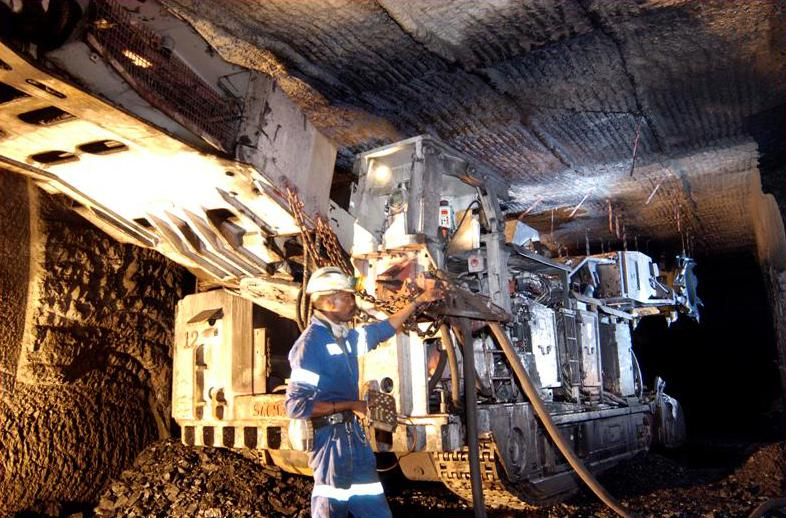
\includegraphics[width=0.7\textwidth]{Continuous_Miner.jpg}
\caption{Continous Miner. 
 The machine operator must stand close to the machine and cutting interface to control the machine.
The operators use many cues, but ultimately must track if they are cutting the target material and 
the state of tool wear. Allowing operators to maintain a greater distance while giving them
the feedback they require can improve production and safety.}
\label{fig:conminer}
\end{figure}

The technologies proposed in this dissertation could be used to automate feedback collection
during the rock cutting process, allowing operators to perform their duties from a safer location.
This work investigates using measured frequency responses to predict material and wear conditions
using a non-linear dynamic capacitive load cell. 
An acoustic tool wear detection method is also developed using this same premise.
The capstone of this project is a custom capacitive load cell that is able to measure 
rock cutting forces using a linear model. 
Each of these three works are respectively summarized in the included journal articles.

This work was sponsored by NIOSH contract 75D30119C05413.
It is a continuation of prior work at Colorado School of Mines \cite{11124/170545}.
The previous work employed piezo electric sensors to make measurements to estimate
rock cutting parameters. 
Our work focuses on use of a capacitive based load cell.
Study of rock fracture mechanics \cite{11124/14359} 
and the effects of tool geometry during rock cutting \cite{11124/13192, 11124/16423, 11124/176345} 
have long been pursued to increase mine efficiency and safety.
By providing an \textit{in-situ} force sensor, this work provides a means
for direct measurement of rock cutting parameters.
In addition to enabling operators to perform their roles from a distance,
this device could also be used to optimize tool geometries 
by providing quick and direct feedback of the cutting forces.

Safety in mines is a serious issue, and the next chapter, Ch.~\ref{chap:2}, discusses its current state.
The chapter after that, Ch.~\ref{chap:3}, covers additional background information regarding sensor choices.
Then, Ch.~\ref{chap:4} discusses modeling of the chosen sensors and materials.
The journal articles that summarize the work are included next. 
Doing rock material type and tool wear classification with a capacitive sensor and 
tool wear classification with an acoustic sensor
are discussed in Chapter \ref{chap:P1} and Chapter \ref{chap:P2}, respectively.
Chapter \ref{chap:P3} discusses the development of the sensor with more linear performance.
Each article describes the implemented classification or regression methods specific to the topic.

After the articles, \ref{chap:8} compares the different capacitive sensor implementations
and discusses the linearity of the final sensor design while providing additional characterization data.
An additional chapter, \ref{chap:9}, describing extensions of the acoustic processing methods is given after that.
The last chapter, \ref{chap:10} highlights the new contributions of this research and gives reccomendations 
for future work and implementation.
This dissertation and the constituent articles have been published as 
Open Access and are released into the public domain.
If you have any questions about this work, you can contact me, the author, at:
austinfoltmanns at gmail dot com with the subject line containing "THESIS".

